\chapter{Camera}
Fino ad ora abbiamo trattato le cosiddette \textbf{matrici di modellazione}, il cui scopo \`e quello di applicare delle
trasformazioni direttamente alla geometria disegnata oppure a qualcuno dei nostri frame.

In questo capitolo tratteremo invece le \textbf{matrici di vista} e le \textbf{matrici di proiezione}. Esse servono ad
applicare trasformazioni al punto di vista o, in gergo, ad effettuare \textbf{movimenti di camera} e creare effetti di
prospettiva differenti tra loro.

\section{Frame per la vista}
Prima di addentrarci nell'argomento dobbiamo precisare che quando si parla di movimenti di camera, il sistema di
riferimento lungo il quale ci muoviamo non \`e quello solito. Mentre per gli assi $x$ e $y$ le cose non cambiano,
l'asse $z$ si sviluppa in maniera inversa.

Di norma, tanto pi\`u grande \`e il valore $z$ di un oggetto, tanto pi\`u questo oggetto si muover\`a "all'interno dello
schermo". Ma nel caso volessimo spostare il punto di vista, ad un valore pi\`u grande di $z$, corrisponderebbe un
allontanamento dalla scena (come se ci stessimo muovendo all'indietro).

\begin{center}
	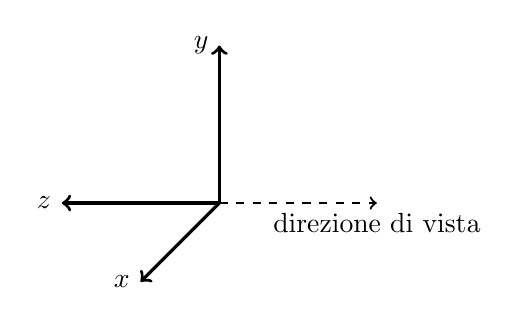
\begin{tikzpicture}[scale=2.0]
		\draw[dashed, thick, ->] (0.0, 0.0) -- (1.0, 0.0) node[below, color=black] {direzione di vista};
		\draw[very thick, ->] (0.0, 0.0) -- (-1.0, 0.0) node[left, color=black] {$z$};
		\draw[very thick, ->] (0.0, 0.0) -- (0.0, 1.0) node[left, color=black] {$y$};
		\draw[very thick, ->] (0.0, 0.0) -- (-0.5, -0.5) node[left, color=black] {$x$};
	\end{tikzpicture}
\end{center}

Bisogna comunque fare attenzione al fatto che questa \`e solo una convenzione. Il vero sistema di riferimento, in cui si
disegna la nostra geometria e nel quale si muove l'osservatore, segue comunque gli assi standard. Dunque, i valori che
useremo per $z$, quando trattiamo i movimenti dell'osservatore, saranno invertiti ma poi dovranno essere svolte le
opportune conversioni per rendere le modifiche consistenti con il frame reale, ossia quello in cui ci stiamo muovendo e
nel quale disegnamo tutta la nostra geometria.

\section{Matrici di proiezione}
Mentre la matrice di vista si occupa di muovere la camera nello spazio la \textbf{matrice di proiezione} definisce il
tipo di camera che stiamo usando.

Ne esistono di due tipi, la prima \`e detta \textbf{prospettica}, la seconda invece \`e detta \textbf{ortogonale}.
Questi due tipi di camera creano due effetti distinti e si prestano per compiti abbastanza differenti.

\subsection{Matrice di proiezione prospettica}
La \textbf{matrice di proiezione prospettica}, come suggerisce il nome, serve a creare l'effetto della prospettiva.
Con questo tipo di camera noi andremo a definire una sorta di cono visivo a partire dal punto in cui \`e posizionata
la camera.

Questo \`e il tipo di camera che ci \`e pi\`u semplice immaginare dato che funziona esattamente come l'occhio umano:
gli oggetti che si allontanano ci appaiono pi\`u piccoli e quelli che che si avvicinano ci appaiono pi\`u grandi.
Si avr\`a inoltre l'effetto prospettico per oggetti che non sono dritti davanti a noi.

\begin{center}
	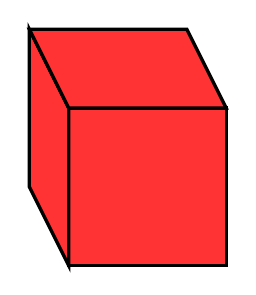
\begin{tikzpicture}
		\filldraw [very thick, color=black, fill=red!80]
		(-1.0, -1.0) --
		(-1.0, 1.0) --
		(1.0, 1.0) --
		(1.0, -1.0) --
		cycle;
		\filldraw [very thick, color=black, fill=red!80]
		(-1.0, -1.0) --
		(-1.5, 0.0) --
		(-1.5, 2.0) --
		(-1.0, 1.0) --
		cycle;
		\filldraw [very thick, color=black, fill=red!80]
		(-1.5, 2.0) --
		(0.5, 2.0) --
		(1.0, 1.0) --
		(-1.0, 1.0) --
		cycle;
	\end{tikzpicture}
\end{center}
